\section{Amplifier circuit}
As the Flexar's coil impedance is 30$\Omega$, and the maximum power they can withstand is 0.8W, the power stage must be able to provide a voltage of about \textbf{6V} at a current of \textbf{0.2A}. \\
Such a high current requires the use of a power amplifier, usually an of the shelf audio amplifier could be used but such devices are built to handle only the audible frequency range (20Hz-20kHz), and our actuators must be able to work between 1Hz and 1kHz which corresponds to the human tactile perception range. \\
A solution is to implement a custom amplifying circuit based on a special type of operational amplifier, the Power OP-AMP.

% -- Subsection 2.1
\subsection{Power Operational Amplifiers}
Power operational amplifiers (power op-amps) are a specialized class of operational amplifiers designed to handle higher current and power levels than standard op-amps. While traditional op-amps are primarily used for signal processing and conditioning in low-power applications, power op-amps are essential for driving heavy loads, including motors, speakers, and other devices that require substantial power. \\
Power op-amps integrate the fundamental principles of conventional op-amps—such as high gain, high input impedance, and low output impedance—with the ability to deliver higher current and power. 

These devices are composed of simple op-amp circuits with a power stage, usually a power transistor, connected to the output of the op-amp. The power stage is responsible for delivering the required current to the load, while the op-amp provides the necessary voltage gain and feedback control. \\
\begin{figure}
    \centering
    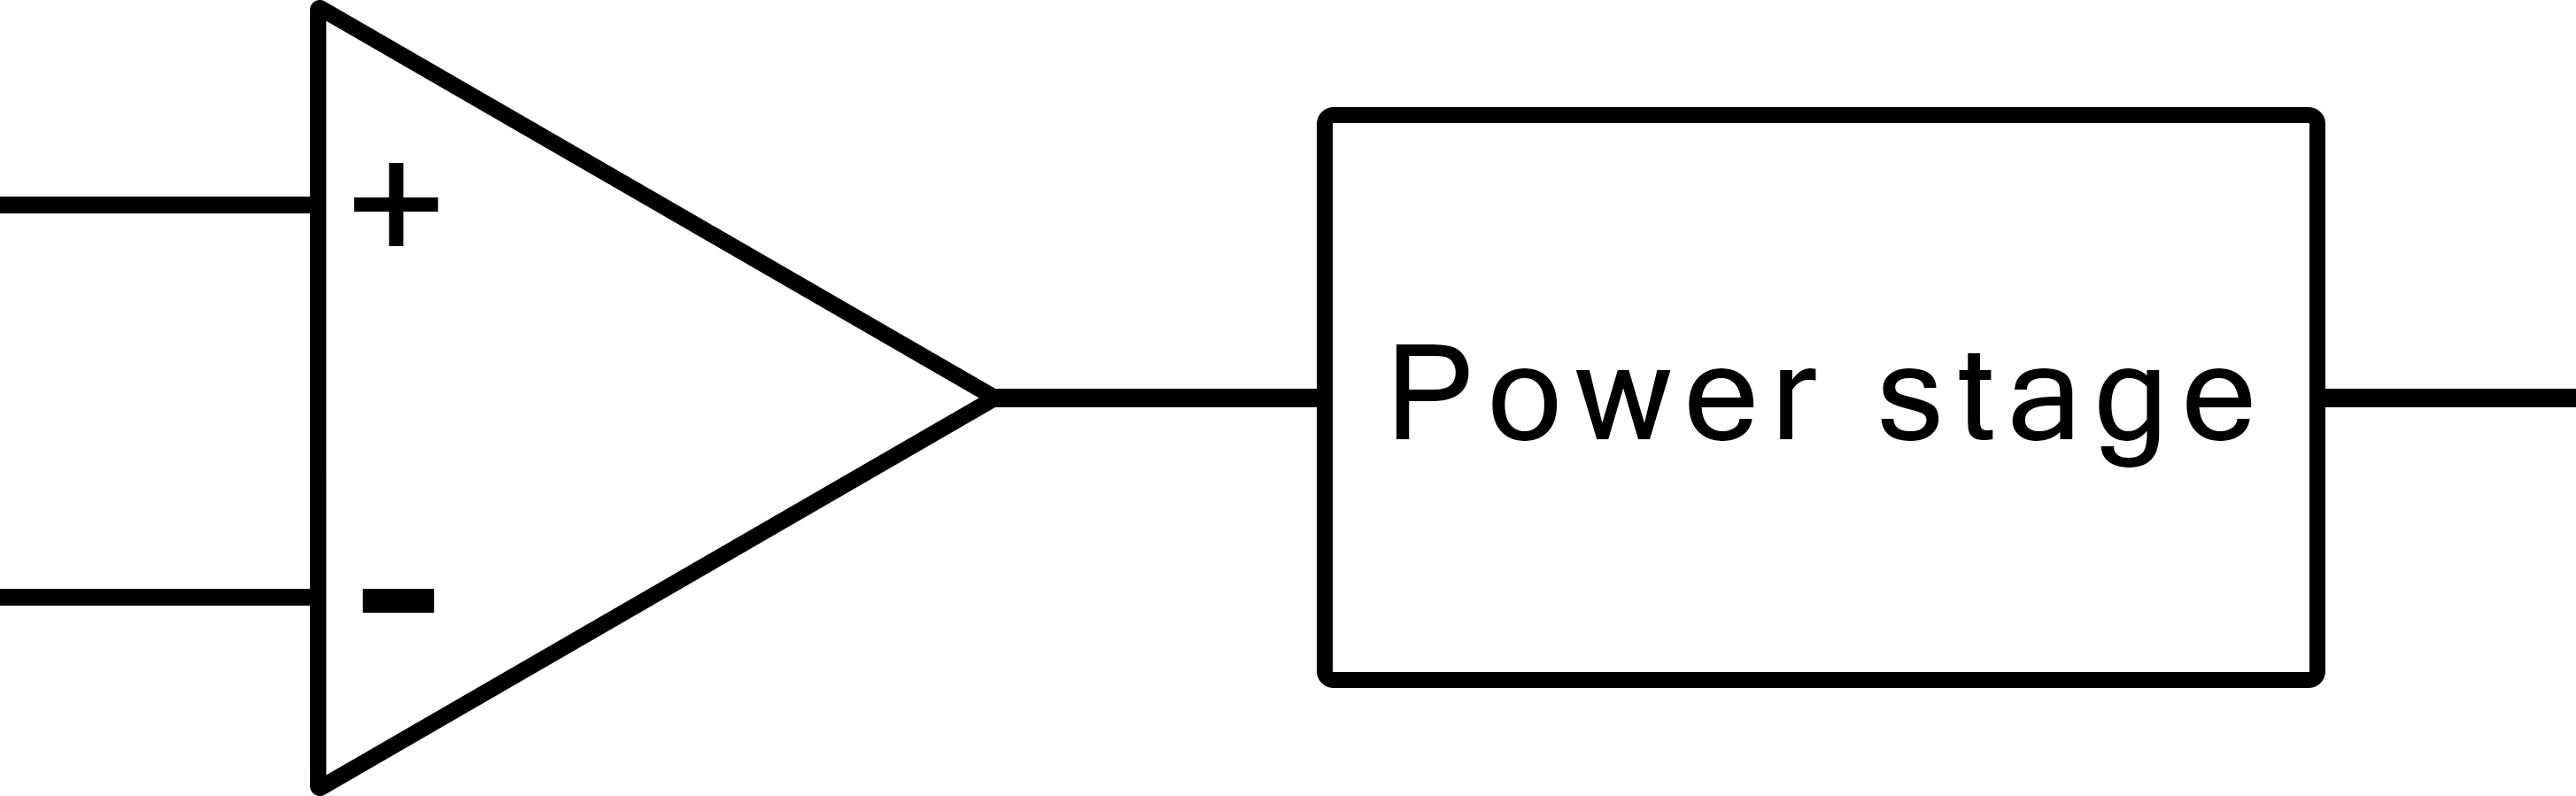
\includegraphics[width=0.5\textwidth]{Chapters/Chapter4/Figures/power_op-amp_block_diagram.png}
    \caption{Power Op Amp block diagram.}
    \label{fig:Power_Op_Amp}
\end{figure}

\subsubsection{Power op-amp characteristics}
Any op-amp that can deliver more than 100mA of current is considered a power op-amp; there exist models that can deliver up to 10A.
For our application, we chose a power op-amp that can deliver up to 1A of current, as it is more than enough to drive the Flexar's coils for simple AC signals.
Another factor for this decision is the high cost of these components, especially at higher current ratings, due to their complexity and the scarcity of requests for this type of component from the market.

The component we landed on is the \textbf{L272} from STMicroelectronics, this small chip can deliver up to a sustained 1A of current, 1.5A of peak current, and can handle a maximum supply voltage of 28V. \\
In dynamic conditions is also to be noted that the L272 has a slew rate of $1\frac{V}{\mu s}$ and, a gain-bandwidth product of 350kHz \cite{L272}.
\subsubsection{Power dissipation problems}
A big problem with power op-amps is the power dissipation, as they are designed to deliver high current levels, they also dissipate a lot of power, which can lead to overheating and damage to the device. \\
For example, the L272 can handle up to 145°C but at only 5W it reaches 75°C, so a heat sink is required to keep the device at a safe temperature.

% -- Subsection 2.2
\subsection{High Power Voltage Amplifier}
As we specified before we decided to implement a power stage with a gain of 10, starting with the circuit of a simple inverting amplifier (the real gain is -10 but for the sake of our application a wave flipped by 180° is acceptable).

\begin{figure}
    \centering
    \resizebox{.7\linewidth}{!}{\begin{circuitikz}
    % Draw the op-amp
    \draw (0,0) node[op amp] (opamp) {};

    % Draw the connection between the + node and the ground
    \draw (opamp.+) -- ++(0,-0.5) node[ground] {};

    % Draw the first resistor to input (l_ is to put the name on top)
    \draw (opamp.-) to[R, l_=$R_1$] ++ (-2,0) to[short, o-] ++ (0,0) node[left]{$V_{in}$} {};

    % Go up one unit and create fb node
    \draw (opamp.-) -- ++ (0,1) coordinate(fb);
    
    % Draw the feedback resistor
    \draw (fb) to[R=$R_f$] ++ (2.5,0) coordinate(end);

    % Draw the connection between the end of Rf and the output of the op-amp, (opamp.out -| end) is the intersection between the vertical line from the output of the op-amp and the horizontal line from the end of Rf
    \draw (end) -- (opamp.out -| end) -- (opamp.out) coordinate(out);

    % Draw the output node 
    \draw (out) to[short, -o] ++ (1,0) node[right]{$V_{out}$} ;
    
\end{circuitikz}}
    \caption{Inverting amplifier circuit.}
    \label{fig:non-inv_ampl}
\end{figure}

The gain can be calculated using the following formula:
\begin{equation}
    A = \frac{V_{out}}{V_{in}} = -\frac{R_f}{R_1}
\end{equation}

Where:
\begin{itemize}
    \item $V_{in}$ is the input voltage.
    \item $V_{out}$ is the output voltage.
    \item $R_1$ is the input resistor.
    \item $R_f$ is the feedback resistor.
\end{itemize}

The values of $R_1$ and $R_f$ have been chosen to be 4.7$k\Omega$ and 47$k\Omega$ respectively, as they are standard values and their order is big enough to work with the provided DAC current of 12mA.

% -- Subsection 2.3
\subsection{Noise filtering}
While implementing the amplifier circuit, we noticed that the output signal had a lot of high-frequency noise, which was not present in the input signal. \\
To solve this problem, we decided to implement a simple low-pass filter adding a capacitor in parallel with the feedback resistor.

\begin{figure}
    \centering
    \resizebox{.7\linewidth}{!}{\begin{circuitikz}
    % Draw the op-amp
    \draw (0,0) node[op amp] (opamp) {};

    % Draw the connection between the + node and the ground
    \draw (opamp.+) -- ++(0,-0.5) node[ground] {};

    % Draw the first resistor to input (l_ is to put the name on top)
    \draw (opamp.-) to[R, l_=$R_1$] ++ (-2,0) to[short, o-] ++ (0,0) node[left]{$V_{in}$} {};

    % Go up one unit and create fb node
    \draw (opamp.-) -- ++ (0,1) coordinate(fb);
    
    % Draw the feedback resistor
    \draw (fb) to[R=$R_f$] ++ (2.5,0) coordinate(end);

    % Draw the capacitor in parallel to Rf
    \draw (fb) -- ++ (0,1.2) to[C=$C_f$] ++ (2.5,0) -- (end);

    % Draw the connection between the end of Rf and the output of the op-amp, (opamp.out -| end) is the intersection between the vertical line from the output of the op-amp and the horizontal line from the end of Rf
    \draw (end) -- (opamp.out -| end) -- (opamp.out) coordinate(out);

    % Draw the output node 
    \draw (out) to[short, -o] ++ (1,0) node[right]{$V_{out}$} ;
    
\end{circuitikz}}
    \caption{Inverting amplifier circuit with low-pass filter.}
    \label{fig:non-inv_ampl_filter}
\end{figure}

The cutoff frequency of the filter can be calculated using the following formula:
\begin{equation}
    f_c = \frac{1}{2\pi R_f C_f}
\end{equation}

Where:
\begin{itemize}
    \item $f_c$ is the cutoff frequency.
    \item $R_f$ is the feedback resistor.
    \item $C_f$ is the capacitor in parallel with the feedback resistor.
\end{itemize}

We set a cutoff frequency of 50kHz, as it is high enough to filter out the noise but low enough to keep the signal intact.
To achieve this, we chose a capacitor of 680pF, as it is a standard value and provides a cutoff frequency of 50kHz with the chosen feedback resistor.

\begin{figure}
    \centering
    \resizebox{.7\linewidth}{!}{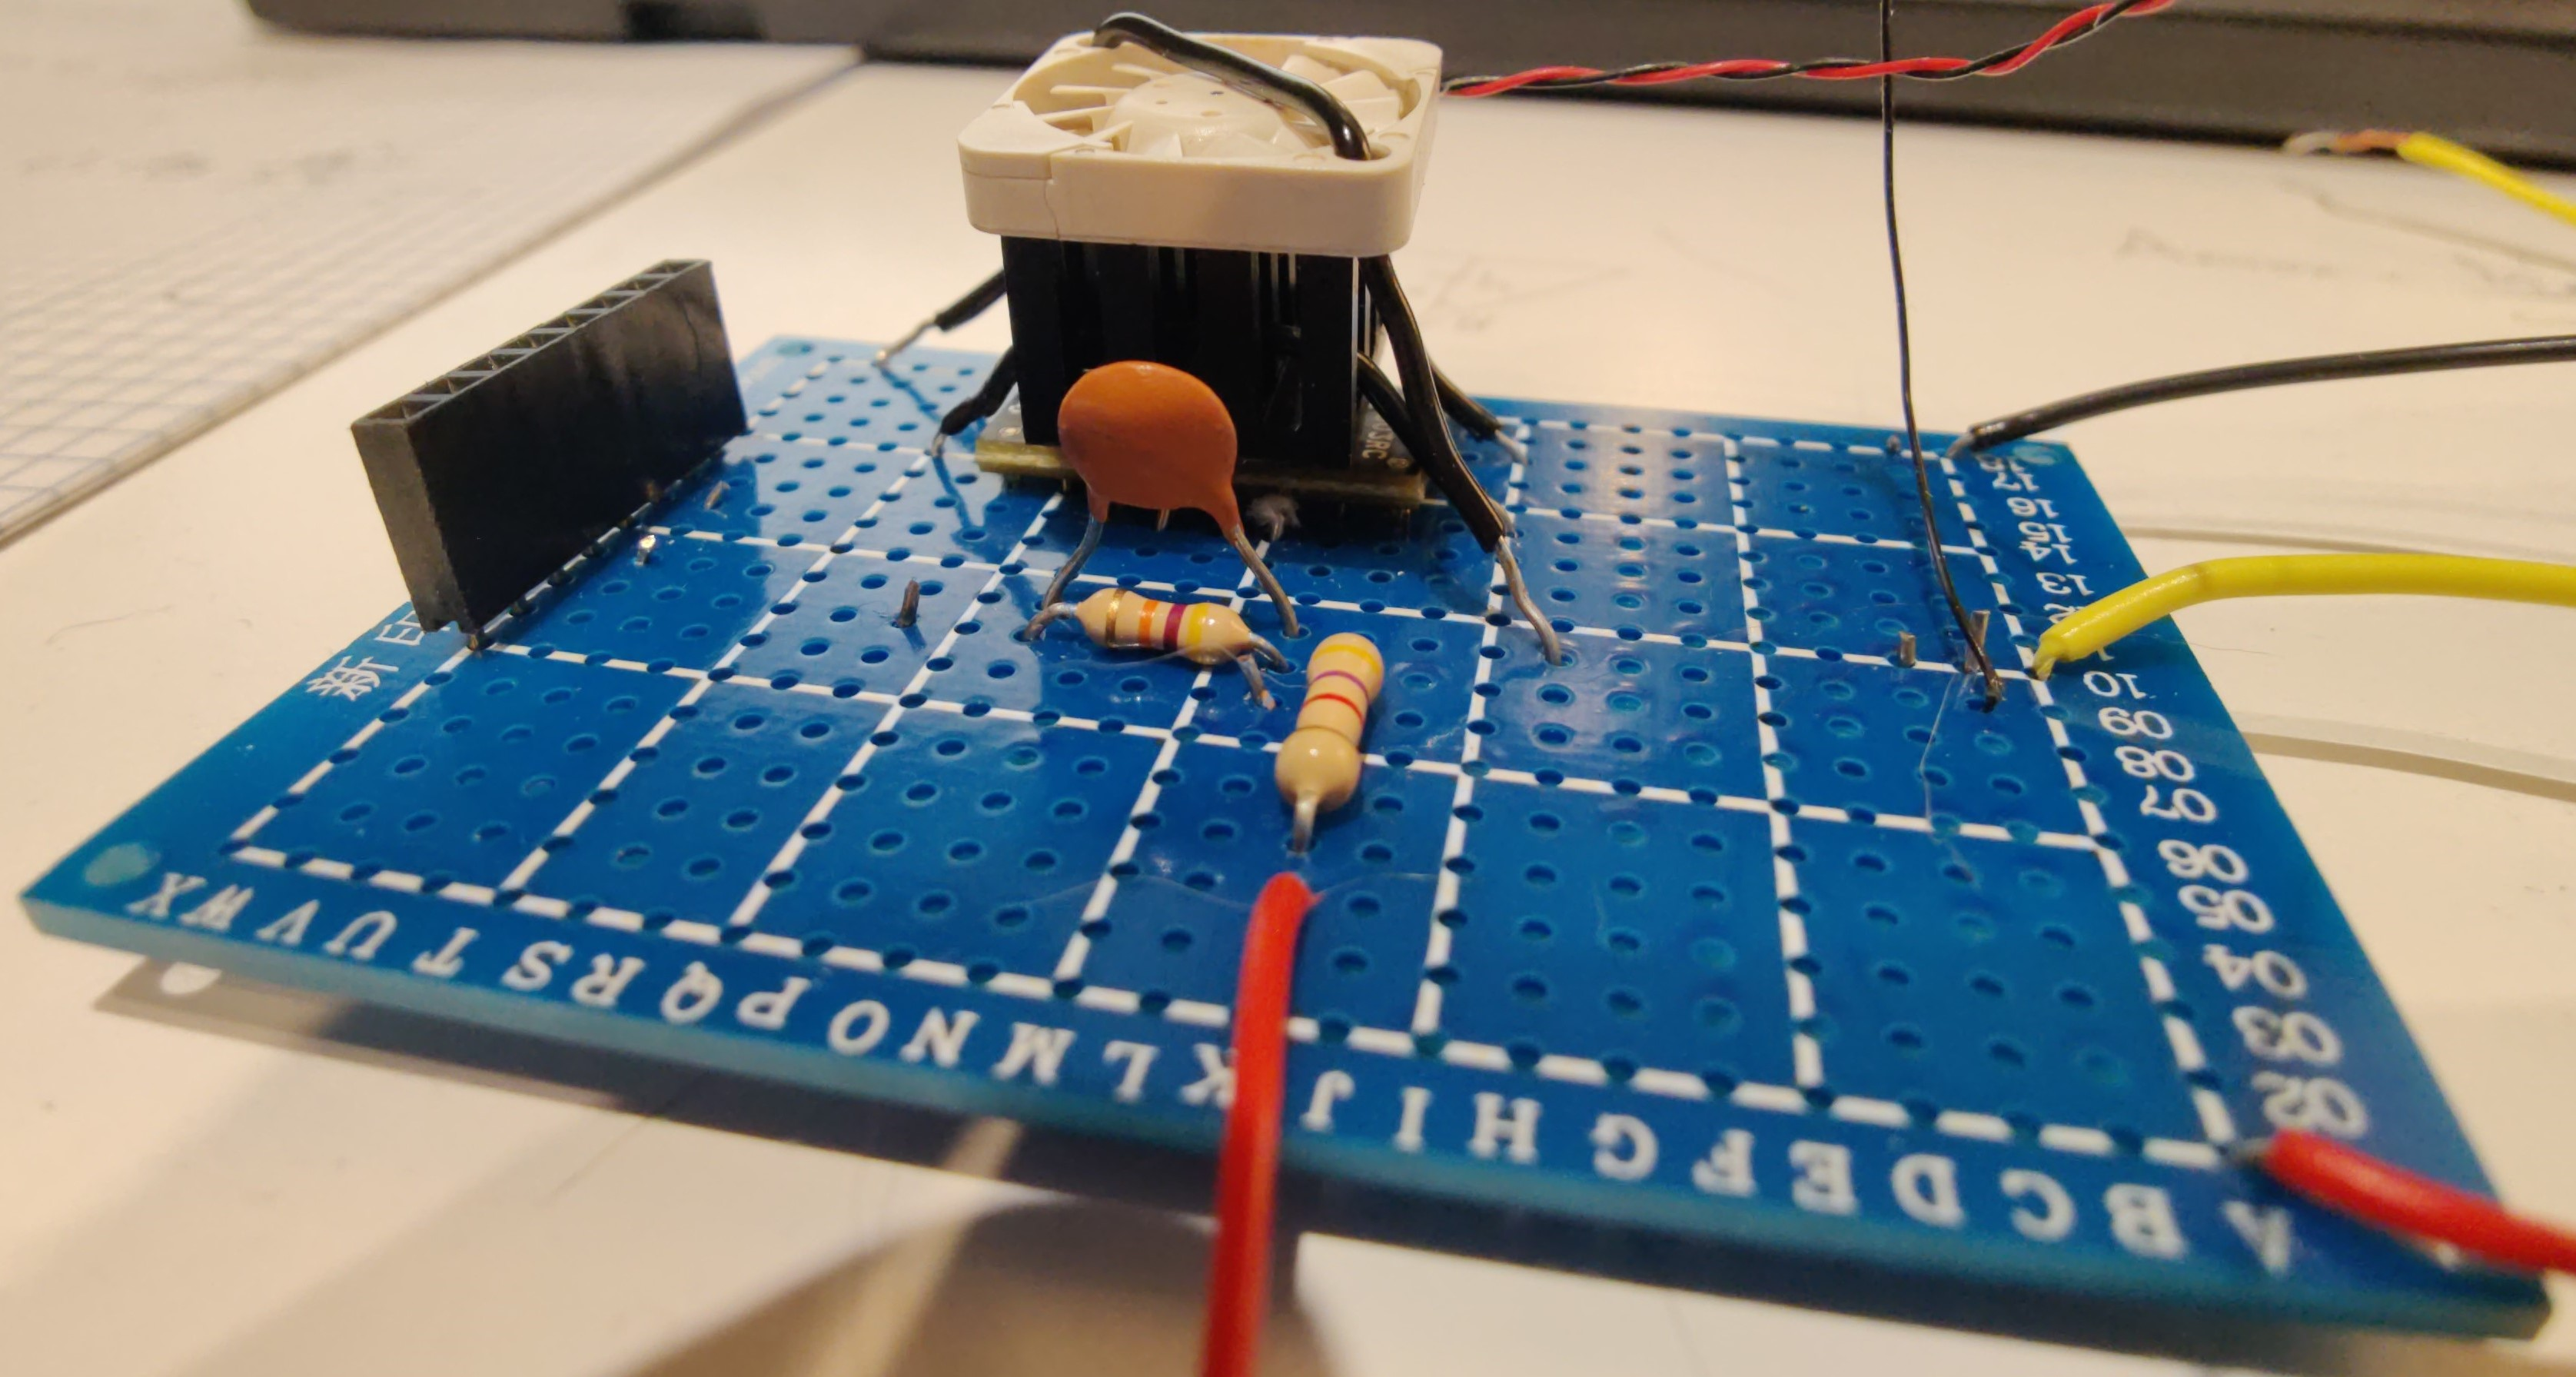
\includegraphics{Chapters/Chapter4/Figures/irl_power_stage.jpg}}
    \caption{Picture of the implemented power stage.}
    \label{fig:IRL_power_stage}
\end{figure}
